\documentclass{beamer}
\usepackage[utf8]{inputenc}
\usetheme{Madrid}
\usecolortheme{default}
\usepackage{amsmath,amssymb,amsfonts,amsthm}
\usepackage{mathtools}
\usepackage{txfonts}
\usepackage{tkz-euclide}
\usepackage{listings}
\usepackage{adjustbox}
\usepackage{array}
\usepackage{tabularx}
\usepackage{gvv}
\usepackage{lmodern}
\usepackage{circuitikz}
\usepackage{tikz}
\usepackage{graphicx}
\setbeamertemplate{page number in head/foot}[totalframenumber]
\usepackage[T1]{fontenc}
\usepackage{tcolorbox}
\tcbuselibrary{minted,breakable,xparse,skins}

\definecolor{bg}{gray}{0.95}
\DeclareTCBListing{mintedbox}{O{}m!O{}}{%
  breakable=true,
  listing engine=minted,
  listing only,
  minted language=#2,
  minted style=default,
  minted options={%
    linenos,
    gobble=0,
    breaklines=true,
    breakafter=,,
    fontsize=\small,
    numbersep=8pt,
    #1},
  boxsep=0pt,
  left skip=0pt,
  right skip=0pt,
  left=25pt,
  right=0pt,
  top=3pt,
  bottom=3pt,
  arc=5pt,
  leftrule=0pt,
  rightrule=0pt,
  bottomrule=2pt,
  toprule=2pt,
  colback=bg,
  colframe=orange!70,
  enhanced,
  overlay={%
    \begin{tcbclipinterior}
    \fill[orange!20!white] (frame.south west) rectangle ([xshift=20pt]frame.north west);
    \end{tcbclipinterior}},
  #3,
}

% Code style
\lstset{
    language=C,
    basicstyle=\ttfamily\small,
    keywordstyle=\color{blue},
    stringstyle=\color{orange},
    commentstyle=\color{green!60!black},
    numbers=left,
    numberstyle=\tiny\color{gray},
    breaklines=true,
    showstringspaces=false,
}

% Title info
\title %optional
{7.4.25}
\date{October 11, 2025}
\author % (optional)
{EE25BTECH11018 - Darisy Sreetej}

\begin{document}

\frame{\titlepage}

\begin{frame}{Question}
The locus of the centre of a circle, which touches the circle is $x^2 + y^2 -6x -6y +14 =0$ and also touches the y-axis, is given by the equation:
\begin{enumerate}
    \item $x^2-6x-10y+14=0$
    \item $x^2-10x-6y+14=0$
    \item $y^2-6x-10y+14=0$
    \item $y^2-10x-6y+14=0$
\end{enumerate}
\end{frame}
\begin{frame}{Solution}
Given circle equation is ,
$$x^2 + y^2 -6x -6y +14 =0$$
can be represented as 
\begin{align}
    \norm{\vec{x}}^2+2\myvec{-3\\-3}^\top\vec{x}+14=0
\end{align}
The centre of circle is $\vec{c}_1=\myvec{3\\3}$ and radius $r=2$ $\brak{\because f= 14 ,\quad \vec{u}=\myvec{-3\\-3}} $\\
Let the centre of the moving circle be $\vec{c}=\myvec{h\\k}$\\
As the circle touches $X-$axis , Distance of a point from $x$-axis is given by
\begin{align}
    R=|\vec{n}^\top\vec{c}|
\end{align}
\end{frame}
\begin{frame}
where $\vec{n}$ is the unit vector normal to $x$-axis\\
\begin{align}
 \vec{n}=\myvec{1\\0}
\end{align}
Distance between their centers equal to sum of their radius
\begin{align}
    \norm{\vec{c}-\vec{c_1}}&=R \pm r\\
\norm{\vec{c}-\vec{c_1}}&=|\vec{n}^\top\vec{c}| \pm r\\
\norm{\vec{c}-\vec{c_1}}^2&=\brak{|\vec{n}^\top\vec{c}| \pm r}^2 
\end{align}
\begin{align}
\brak{\vec{c}-\vec{c_1}}\brak{\vec{c}-\vec{c_1}}^\top=\brak{|\vec{n}^\top\vec{c}| \pm r}^2 
\end{align}
\begin{align}
\vec{c}^\top\vec{c}+\vec{c_1}\vec{c_1}^\top-\vec{c_1}^\top\vec{c}-\vec{c}^\top\vec{c_1}&= \brak{|\vec{n}^\top\vec{c}|}^2 \pm 2r|\vec{n}^\top\vec{c}|+r^2\\
\vec{c}^\top\vec{c}+\vec{c_1}\vec{c_1}^\top-\vec{c_1}^\top\vec{c}-\vec{c}^\top\vec{c_1}&= \brak{\vec{n}^\top\vec{c}}^\top\brak{\vec{n}^\top\vec{c}}  \pm 2r|\vec{n}^\top\vec{c}|+r^2\\
\vec{c}^\top\vec{c}+\norm{\vec{c_1}}^2-2\vec{c_1}^\top\vec{c}&=\brak{\vec{c}^\top\vec{n}\vec{n}^\top\vec{c}} \pm 2r|\vec{n}^\top\vec{c}|+ r^2
\end{align}
\end{frame}
\begin{frame}
 \begin{align}
\vec{c}^\top\vec{c}+18&=\brak{\vec{c}^\top\vec{n}\vec{n}^\top\vec{c}}+2\vec{n}^\top\vec{c} \pm 2r|\vec{n}^\top\vec{c}|+ r^2 + 2\vec{c_1}^\top\vec{c}\\
\vec{c}^\top\vec{c}+14&=\brak{\vec{c}^\top\vec{n}\vec{n}^\top\vec{c}}+2\vec{n}^\top\vec{c} \pm 4|\vec{n}^\top\vec{c}| + 2\vec{c_1}^\top\vec{c}  \quad (\text{Since r=2})
\end{align}
\textbf{Case 1} : (External Tangency)
\begin{align}
\vec{c}^\top\vec{c}+14&=\brak{\vec{c}^\top\vec{n}\vec{n}^\top\vec{c}}+2\vec{n}^\top\vec{c} + 4|\vec{n}^\top\vec{c}| + 2\vec{c_1}^\top\vec{c}
\end{align}
\begin{align}
\myvec{x&y}\myvec{x\\y} +14 = \myvec{x&0}\myvec{x\\0} + 4 \brak{\myvec{1 & 0}\myvec{x\\y}} + 2\brak{\myvec{3&3}\myvec{x\\y}}
\end{align}
\begin{align}
x^2+y^2+14=x^2+4x+6x+6y\\
y^2-10x-6y+14=0
\end{align}
\end{frame}
\begin{frame}
\textbf{Case 2} : (Internal Tangency)
\begin{align}
\vec{c}^\top\vec{c}+14&=\brak{\vec{c}^\top\vec{n}\vec{n}^\top\vec{c}}+2\vec{n}^\top\vec{c} - 4|\vec{n}^\top\vec{c}| + 2\vec{c_1}^\top\vec{c}
\end{align}
\begin{align}
\myvec{x&y}\myvec{x\\y} +14 = \myvec{x&0}\myvec{x\\0} - 4 \brak{\myvec{1 & 0}\myvec{x\\y}} + 2\brak{\myvec{3&3}\myvec{x\\y}}
\end{align}
\begin{align}
x^2+y^2+14=x^2-4x+6x+6y\\
y^2-2x-6y+14=0
\end{align}
Therefore , the locus of the centre of a circle is 
$$
 y^2-10x-6y+14=0   \quad  (\text{from the options})
$$
\end{frame}
\begin{frame}{Conclusion}
    \text{Hence, option (4) is correct.}
\end{frame}
\begin{frame}{Plot}
\begin{figure}[H]
    \centering
    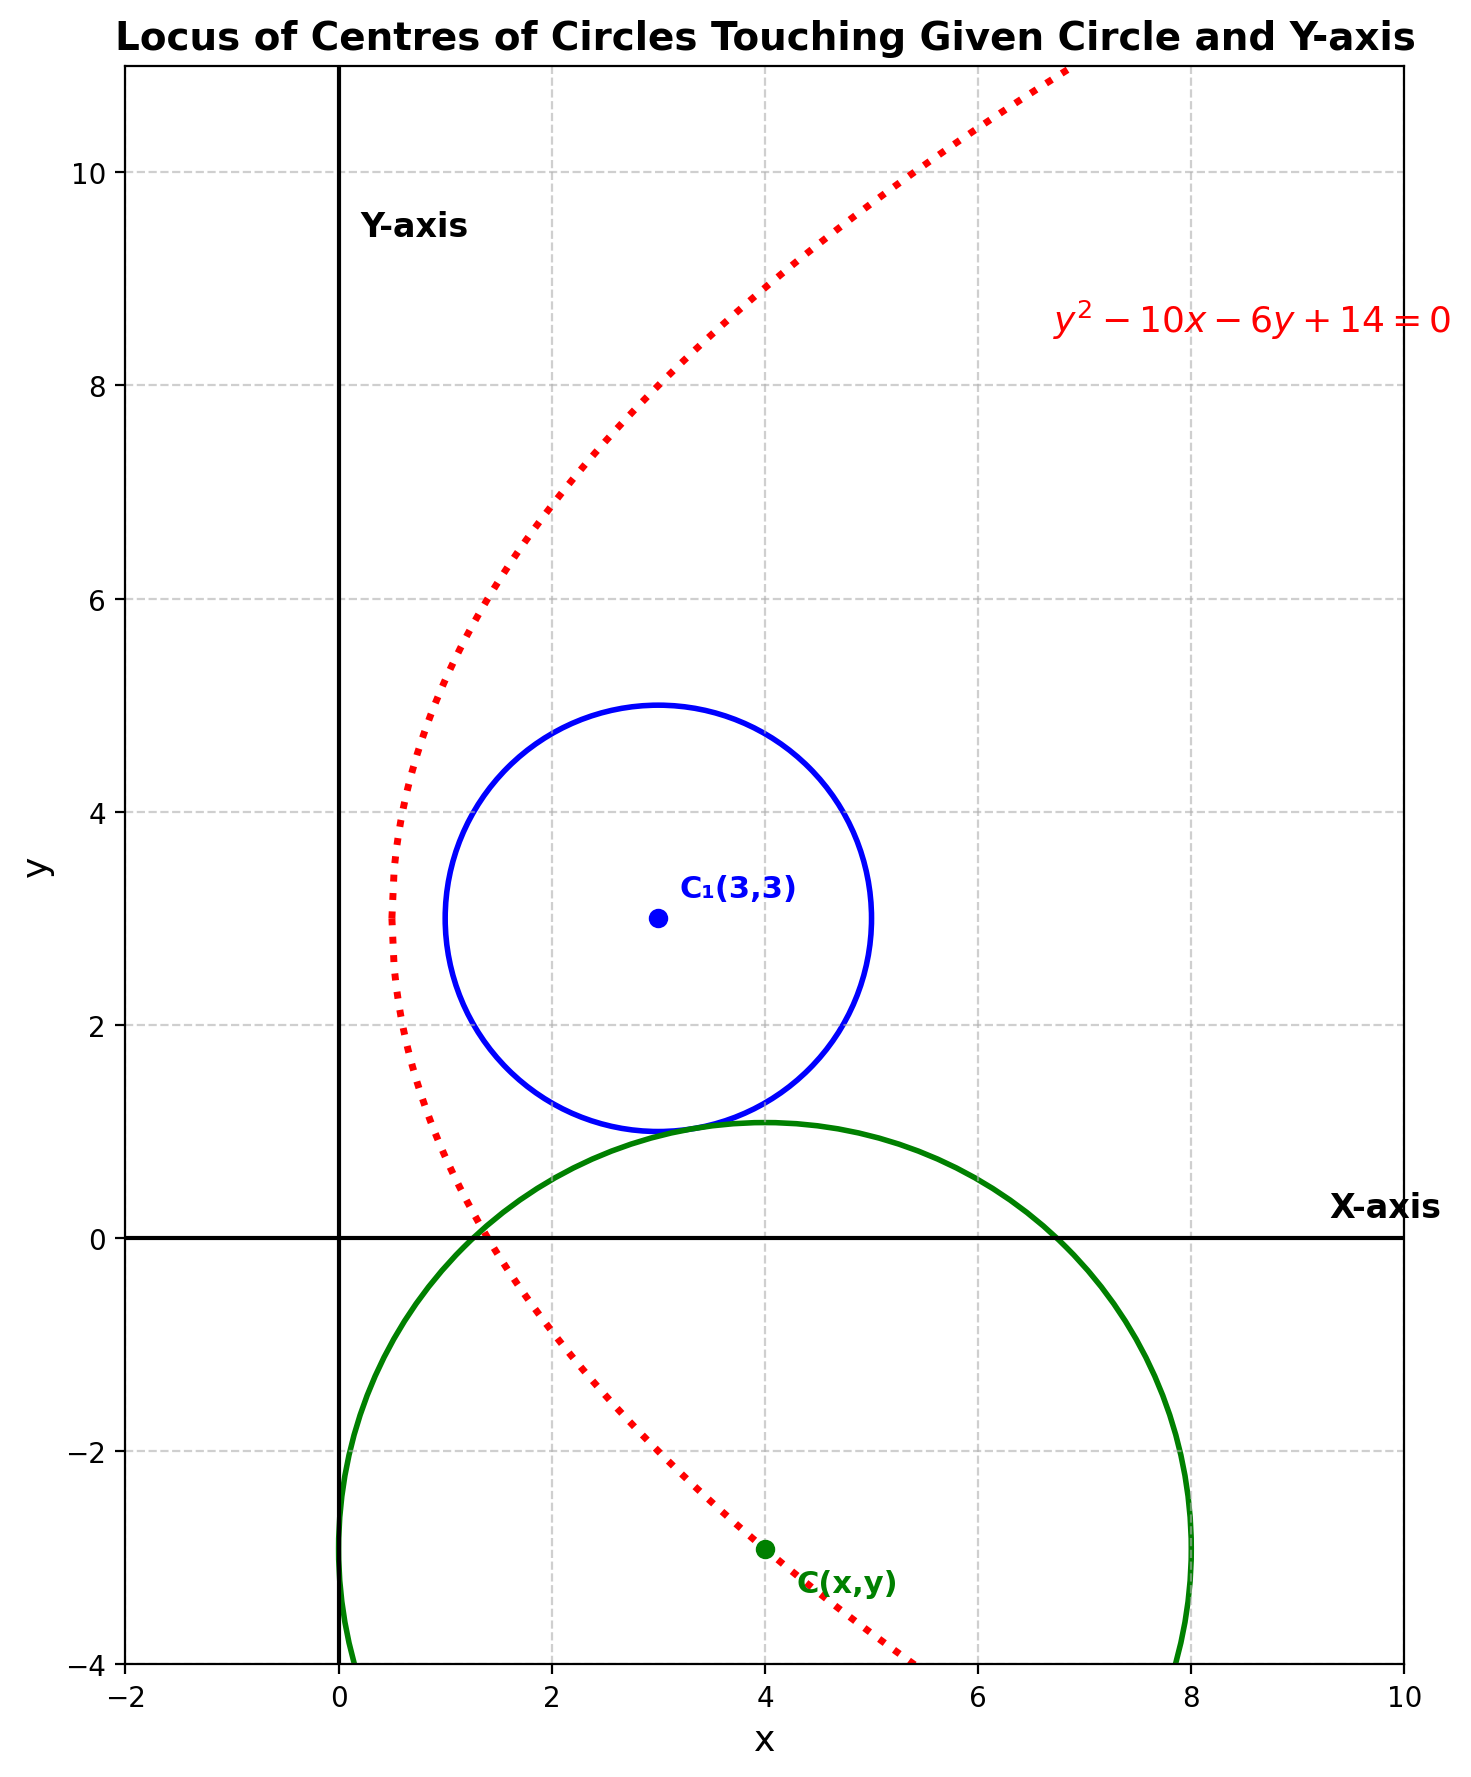
\includegraphics[width=0.5\linewidth]{figs/fig.png}
    \label{fig:placeholder}
\end{figure}
\end{frame}
\begin{frame}[fragile]
\frametitle{C code}
    \begin{lstlisting}[language=C]

#include <stdio.h>

void get_circle_params(double* out_data) {
    // Given circle: x^2 + y^2 - 6x - 6y + 14 = 0
    // Centre: (3,3), radius = 2
    out_data[0] = 3.0;   // x-coordinate
    out_data[1] = 3.0;   // y-coordinate
    out_data[2] = 2.0;   // radius
}
\end{lstlisting}
\end{frame}
\begin{frame}[fragile]
    \frametitle{Python + C code}

    \begin{lstlisting}[language=Python]
import ctypes
import sympy

def find_locus_equation():
    lib = ctypes.CDLL('./code.so')

    double_array_3 = ctypes.c_double * 3
    lib.get_circle_params.argtypes = [ctypes.POINTER(ctypes.c_double)]
    out_data_c = double_array_3()

    lib.get_circle_params(out_data_c)
    c1_x, c1_y, r1 = list(out_data_c)  # c1_x=3.0, c1_y=3.0, r1=2.0

    # Symbols: h,k for centre of variable circle
    h, k = sympy.symbols('h k', real=True)
\end{lstlisting}
\end{frame}
\begin{frame}[fragile]
    \frametitle{Python + C code}

    \begin{lstlisting}[language=Python]
    # We take external tangency and assume h >= 0 => r = h
    r = h

    lhs = (h - c1_x)**2 + (k - c1_y)**2
    rhs = (r + r1)**2

    equation = sympy.Eq(lhs, rhs)
    locus_expr = sympy.simplify(equation.lhs - equation.rhs)

    # Rename symbols to conventional x,y for the returned equation
    x, y = sympy.symbols('x y', real=True)
    final_locus = sympy.simplify(locus_expr.subs({h: x, k: y}))

    return sympy.Eq(final_locus, 0)
\end{lstlisting}
\end{frame}
\begin{frame}[fragile]
\frametitle{Python + C code}
    \begin{lstlisting}[language=Python]
if __name__ == '__main__':
    eq = find_locus_equation()
    print("Derived locus equation:", eq)det_val = lib.determinant(Y)
    \end{lstlisting}
\end{frame}
\begin{frame}[fragile]
\frametitle{Python code}
    \begin{lstlisting}[language=Python]
import sys
sys.path.insert(0, './')
import numpy as np
import matplotlib.pyplot as plt
from call import find_locus_equation

# Get the locus equation
locus_equation = find_locus_equation()
print(f"Locus equation: {locus_equation}")
fig, ax = plt.subplots(figsize=(9, 9))

# Given circle: x² + y² - 6x - 6y + 14 = 0
given_center = (3, 3)
given_radius = 2
given_circle = plt.Circle(given_center, given_radius, color='blue', fill=False, linewidth=2)
ax.add_patch(given_circle)
     \end{lstlisting}
\end{frame}
\begin{frame}[fragile]
\frametitle{Python code}
    \begin{lstlisting}[language=Python]
    # Mark the moving circle centre
ax.plot(x_sample, y_sample, 'go')
ax.text(x_sample + 0.3, y_sample - 0.4, "C(x,y)", color='green', fontsize=11, fontweight='bold')

# Mark centre of given circle
ax.plot(*given_center, 'bo')
ax.text(given_center[0] + 0.2, given_center[1] + 0.2, "C₁(3,3)", color='blue', fontsize=11, fontweight='bold')

# Locus (Parabola):
x_vals = np.linspace(0.5, 9, 400)
sqrt_term = np.sqrt(np.maximum(0, 5 * (2 * x_vals - 1)))
y_plus = 3 + sqrt_term
y_minus = 3 - sqrt_term
ax.plot(x_vals, y_plus, 'r:', linewidth=2.5)
ax.plot(x_vals, y_minus, 'r:', linewidth=2.5)
       \end{lstlisting}
\end{frame}
\begin{frame}[fragile]
\frametitle{Python code}
    \begin{lstlisting}[language=Python]
# Write the parabola equation neatly near the curve
ax.text(6.7, 8.5, r"$y^2 - 10x - 6y + 14 = 0$", color='red', fontsize=13, fontweight='bold')

# Moving circle 
x_sample = 4
y_sample = 3 - np.sqrt(5 * (2 * x_sample - 1))
r_sample = x_sample  # because circle touches y-axis → r = x
moving_circle = plt.Circle((x_sample, y_sample), r_sample, color='green', fill=False, linewidth=2)
ax.add_patch(moving_circle)

# Formatting , Axes setup
ax.axvline(0, color='black', linestyle='-', linewidth=1.5)
ax.axhline(0, color='black', linestyle='-', linewidth=1.5)
ax.text(9.3, 0.2, "X-axis", fontsize=12, fontweight='bold')
ax.text(0.2, 9.4, "Y-axis", fontsize=12, fontweight='bold')
ax.set_xlim(-2, 10)
     \end{lstlisting}
\end{frame}
\begin{frame}[fragile]
\frametitle{Python code}
    \begin{lstlisting}[language=Python]

ax.set_ylim(-4, 11)
ax.set_aspect('equal', 'box')
ax.set_xlabel("x", fontsize=13)
ax.set_ylabel("y", fontsize=13)
ax.set_title("Locus of Centres of Circles Touching Given Circle and Y-axis", fontsize=14, fontweight='bold')
ax.grid(True, linestyle='--', alpha=0.6)

# Save and show
plt.tight_layout()
plt.savefig('fig.png', dpi=200, bbox_inches='tight')
plt.show()
       \end{lstlisting}
\end{frame}
\end{document}
